\begin{frame}{Aucun(e), un(e) ou plusieurs?}
  Avec un(e) partenaire, discute de combien de chaque chose tu as.
  Pose la question dans le modèle à ton/ta partenaire pour chaque numéro.
  \begin{columns}
    \column{0.5\textwidth}
      \small
      \begin{description}
        \item[] \textbf{Modèle:} \emph{petit ami}
        \item[E1:] Est-ce que tu as un petit ami ou plus?
        \item[E2:] Je n'ai aucun petit ami.
        \item[OU] J'ai un petit ami.
        \item[OU] J'ai \alert{quatre} petit\textcolor{red}{s} ami\textcolor{red}{s}!
      \end{description}
      \begin{center}
        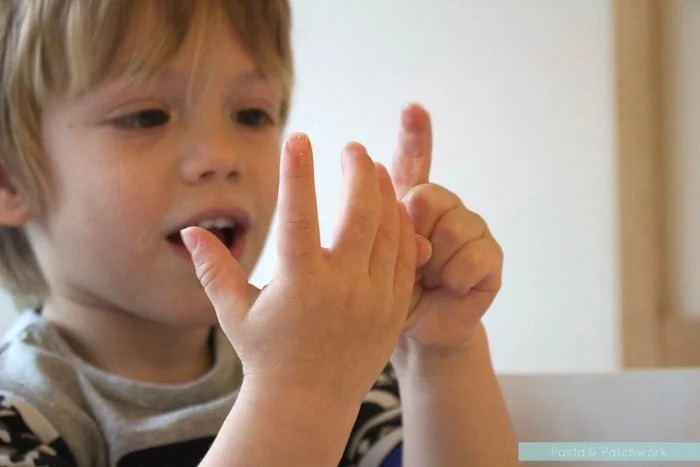
\includegraphics[scale=0.125]{doigts.jpg} \\
        \tiny
        Je compte sur vous, les doigts!
      \end{center}
    \column{0.25\textwidth}
      \begin{enumerate}
        \item bureau
        \item jeu
        \item chou
        \item professeur
        \item sou
        \item cheval
      \end{enumerate}
    \column{0.25\textwidth}
      \begin{enumerate}
        \setcounter{enumi}{6}
        \item œil
        \item emploi
        \item cheveu
        \item couteau
        \item journal
        \item[] \ 
      \end{enumerate}
  \end{columns}
\end{frame}